 % The main file for CAMP reports
 % Don't put any content in here. 
 % Don't even include content files by using \input or \inlcude. 
 % Put your content to TEXT.TEX or include it there using \input.
 % Uses:
 %		SETTINGS.TEX	contains the settings for this document
 %		COMMANDS.TEX	contains commands which can be used while writing
 %		INFO.TEX			contains the author, title and so on for the cover
 %		COVER.TEX			formats the front cover of the document
 %		ABSTRACT.TEX	contains the abstract to be included (if needed)
 %		TEXT.TEX			contains the actual content of the document
 %		BIB.BIB				containt the BibTeX entries for the document
 
 
%% Draft document mode
%% Final document
\documentclass[11pt,a4paper,bibtotoc,idxtotoc,headsepline,footsepline,footexclude,BCOR12mm,DIV13]{scrbook}

%\documentclass[11pt,a4paper,bibtotoc,idxtotoc,headsepline,footsepline,footexclude,BCOR20mm,DIV10]{scrbook}

% KOMA-Optionen:
%  bibtotoc: include bibliography in table of contents
%  idxtotoc: include index in table of contents
%  headsepline: use horizontalline under heading
%  BCOR: binding correcion (Bindungskorrektur) (e.g.: BCOR5mm)
%  DIV: Number of sheet sections (used for layout) (e.g.: DIV12) 



% include title and author information for the cover
% Set here the title, authors and other stuff to be used for the cover
% This file is used by MAIN.TEX

% set title, authors and stuff for the cover
\def\doctype{Bachelorarbeit in Informatik}
\def\title{Object detection and segmentation in cluttered scenes through perception and manipulation}
\def\titleGer{Objekterkennung und Segmentierung durch Perzeption und Manipulation}
\def\author{Julius Adorf}
\def\date{July 15, 2011}

% text to appear in the footer
\def\footertext{}


% include settings
% Included by MAIN.TEX
% Defines the settings for the CAMP report document

\renewcommand{\sectfont}{\normalfont \bfseries}        % Schriftart der Kopfzeile

% manipulate footer
\usepackage{scrpage2}
\pagestyle{scrheadings}
\ifoot[\footertext]{\footertext} % \footertext set in INFO.TEX
%\setkomafont{pagehead}{\normalfont\rmfamily}
\setkomafont{pagenumber}{\normalfont\rmfamily}

%% allow sophisticated control structures
\usepackage{ifthen}

% use Palatino as default font
\usepackage{palatino}

% enable special PostScript fonts
\usepackage{pifont}

% make thumbnails
\usepackage{thumbpdf}

%to use the subfigures
\usepackage{subfigure}


\usepackage{colortbl}


%% show program code\ldots
%\usepackage{verbatim}
%\usepackage{program}

%% enable TUM symbols on title page
\usepackage{styles/tumlogo}


\usepackage{multirow}

%% use colors
\usepackage{color}

%% make fancy math
\usepackage{amsmath}
\usepackage{amsfonts}
\usepackage{amssymb}
% mathtools necessary for dcases environment
% TODO: either remove mathtools.sty from styles or remove install statement in Makefile for texlive-latex3
\usepackage{styles/mathtools}
\usepackage{textcomp}
\usepackage{styles/yhmath} % f�r die adots 
%% mark text as preliminary
%\usepackage[draft,german,scrtime]{prelim2e}

%% create an index
\usepackage{makeidx}


% for the program environment
\usepackage{float}

%% load german babel package for german abstract
%\usepackage[german,american]{babel}
\usepackage[german,english]{babel}
\selectlanguage{english}

% use german characters as well
\usepackage[utf8]{inputenc}       % allow Latin1 characters

% use initals dropped caps - doesn't work with PDF
\usepackage{styles/dropping} % fix

\usepackage{styles/shortoverview}
%----------------------------------------------------
%      Graphics and Hyperlinks
%----------------------------------------------------

%% check for pdfTeX
\ifx\pdftexversion\undefined
 %% use PostScript graphics
 \usepackage[dvips]{graphicx}
 \DeclareGraphicsExtensions{.eps,.epsi}
 \graphicspath{{figures/}{figures/review}} 
 %% allow rotations
 \usepackage{rotating}
 %% mark pages as draft copies
 %\usepackage[english,all,light]{draftcopy}
 %% use hypertex version of hyperref
 \usepackage[hypertex,hyperindex=false,colorlinks=false]{hyperref}
\else %% reduce output size \pdfcompresslevel=9
 %% declare pdfinfo
 %\pdfinfo { 
 %  /Title (my title) 
 %  /Creator (pdfLaTeX) 
 %  /Author (my name) 
 %  /Subject (my subject	) 
 %  /Keywords (my keywords)
 %}
 %% use pdf or jpg graphics
 \usepackage[pdftex]{graphicx}
 \DeclareGraphicsExtensions{.jpg,.JPG,.png,.pdf,.eps}
 \graphicspath{{figures/}} 
 
 %% Load float package, for enabling floating extensions
 \usepackage{float}
 
 %% allow rotations
 \usepackage{rotating}
 %% use pdftex version of hyperref
 \usepackage[pdftex,colorlinks=true,linkcolor=red,citecolor=red,%
 anchorcolor=red,urlcolor=red,bookmarks=true,%
 bookmarksopen=true,bookmarksopenlevel=0,plainpages=false%
 bookmarksnumbered=true,hyperindex=false,pdfstartview=%
 ]{hyperref}
%
%\usepackage[pdftex,colorlinks=false,linkcolor=red,citecolor=red,%
% anchorcolor=red,urlcolor=red,bookmarks=true,%
% bookmarksopen=true,bookmarksopenlevel=0,plainpages=false%
% bookmarksnumbered=true,hyperindex=false,pdfstartview=%
% ]{hyperref}
\fi

%% Fancy chapters
%\usepackage[Lenny]{fncychap}
%\usepackage[Glenn]{fncychap}
%\usepackage[Bjarne]{fncychap}

%\usepackage[avantgarde]{quotchap}

% set the bibliography style
%\bibliographystyle{styles/bauermaNum}
%\bibliographystyle{alpha}
%\bibliographystyle{plain}
\bibliographystyle{ieeetr} % list citations in order of appearance

% Arnold Schwarzenegger trick: can be used to add some flexible space after
% command without the necessity of adding curly brackets when calling the
% command.
% see: http://stackoverflow.com/questions/512729/space-after-latex-commands
\usepackage{xspace}  



% include commands
% Commands to be used within the TUM report document
% Included by MAIN.TEX
% Please include your own cool commands here. 
% Be only sure to comment it sufficiently so others can use it.

%-------------------------------------------------------------
%                      Own Commands
%-------------------------------------------------------------

\newcommand{\clutseg}{{\tt CLUTSEG}\xspace} 	
\newcommand{\tod}{{\tt TOD}\xspace} 	
\newcommand{\oTvh}{_{o}\hat{T}^{v}}
\newcommand{\oTv}{_{o}T^{v}}
\newcommand{\vTo}{_{v}T^{o}} 	
\newcommand{\oTvi}[1]{_{o}T_{#1}^{v}} 	
\newcommand{\vToi}[1]{_{v}T_{#1}^{o}} 	
\newcommand{\fTv}{_{f}T^{v}}
\renewcommand{\vec}[1]{\mathbf{#1}}
\newcommand{\normtwo}[1]{{\left|\left| #1 \right|\right|}_{\mbox{\tiny 2}}} 	
\newcommand{\assamTea}{{\it assam\_tea}\xspace}
\newcommand{\haltbareMilch}{{\it haltbare\_milch}\xspace}
\newcommand{\jacobsCoffee}{{\it jacobs\_coffee}\xspace}
\newcommand{\icedtea}{{\it icedtea}\xspace}

%-------------------------------------------------------------
% math stuff -------------------------------------------------

% nice R, N, C
\newcommand{\nat}{\mathbb{N}}
\newcommand{\real}{\mathbb{R}}
\newcommand{\compl}{\mathbb{C}}



% norm
\newcommand{\norm}[1]{\left\| #1 \right\|}

% un demi
\newcommand{\half}{\frac{1}{2}}

% parantheses
\newcommand{\pth}[1]{ \left( #1 \right) }
\newcommand{\brt}[1]{ \left[ #1 \right] }
\newcommand{\cbr}[1]{ \left\{ #1 \right\} }
%\newcommand{\angle}[1]{ \left\langle  #1 \right\rangle }

% partial derivative: %#1 function, #2 which variable
% simple / single line version
\newcommand{\pardevS}[2]{ \delta_{#1} f(#2) }
% fraction version
\newcommand{\pardevF}[2]{ \frac{\partial #1}{\partial #2} }

% render vectors: 3 and 4 dimensional
\newcommand{\veciii}[3]{\left[ \begin{array}[h]{c} #1 \\ #2 \\ #3	\end{array} \right]}
\newcommand{\veciv}[4]{\left[ \begin{array}[h]{c} #1 \\ #2 \\ #3 \\ #4	\end{array} \right]}

% render matrices: 3  dimensional (arguments in row first order)
\newcommand{\matiii}[9]{\left[ \begin{array}[h]{ccc} #1 & #2 & #3 \\ #4 & #5 & #6 \\ #7 & #8 & #9	\end{array} \right]}
%DOESN'T WORK,DON'T KNOW WHY \newcommand{\mativ}[16]{\left[ \begin{array}[h]{cccc} #1 & #2 & #3 & #4 \\ #5 & #6 & #7 & #8 \\ #9 & #10 & #11 & #12 \\ #13 & #14 & #15 & #16 \end{array} \right]}


%-------------------------------------------------------------
%-------------------------------------------------------------


%-------------------------------------------------------------
% some abreviations ------------------------------------------
\newcommand{\Reg}{$^{\textregistered}$}
\newcommand{\reg}{$^{\textregistered}$ }
\newcommand{\Tm}{\texttrademark}
\newcommand{\tm}{\texttrademark~}
\newcommand {\bsl} {$\backslash$}

%-------------------------------------------------------------
%-------------------------------------------------------------


%-------------------------------------------------------------
% formating --------------------------------------------------

% Theorem & Co environments and counters
\newtheorem{theorem}{Theorem}[chapter]
\newtheorem{lemma}[theorem]{Lemma}
\newtheorem{corollary}[theorem]{Corollary}
\newtheorem{remark}[theorem]{Remark}
\newtheorem{definition}[theorem]{Definition}
\newtheorem{equat}[theorem]{Equation}
\newtheorem{example}[theorem]{Example}
\newtheorem{algorithm}[theorem]{Algorithm}

% inserting figures
\newcommand{\insertfigure}[4]{ % Filename, Caption, Label, Width percent of textwidth
	\begin{figure}[htbp]
		\begin{center}
			\includegraphics[width=#4\textwidth]{#1}
		\end{center}
		\vspace{-0.4cm}
		\caption{#2}
		\label{#3}
	\end{figure}
}




% referencing figures

\newcommand{\refFigure}[1]{ %label
	Figure~\ref{#1}
}
\newcommand{\refChapter}[1]{ %label
	Chapter~\ref{#1}
}

\newcommand{\refSection}[1]{ %label
	Section~\ref{#1}
}

\newcommand{\refParagraph}[1]{ %label
	Paragraph~\ref{#1}
}

\newcommand{\refEquation}[1]{ %label
	Equation~\ref{#1}
}

\newcommand{\refTable}[1]{ %label
	Table~\ref{#1}
}




\newcommand{\rigidTransform}[2]
{
	${}^{#2}\!\vec{H}_{#1}$
}

%code, in typewriter
\newcommand{\code}[1]
 {\texttt{#1}}

% comment that appears on the border - very practical !!!
\newcommand{\comment}[1]{\marginpar{\raggedright \noindent \footnotesize {\sl #1} }}

% page clearing
\newcommand{\clearemptydoublepage}{%
  \ifthenelse{\boolean{@twoside}}{\newpage{\pagestyle{empty}\cleardoublepage}}%
  {\clearpage}}


%-------------------------------------------------------------
%-------------------------------------------------------------


\newcommand{\etAl}{\emph{et al.}\mbox{ }}



%\makeindex
	%% inter line spacing
%\linespread{1.0}

\makeglossary

\begin{document}

	\frontmatter
	
	
	% The front cover for the TUM report document.
% Included by MAIN.TEX


%--------------------------------------------------
% The Front Cover
%--------------------------------------------------

% The front cover for the TUM document.
% Included by MAIN.TEX


%--------------------------------------------------
% The Front Cover
%--------------------------------------------------

% correct BCOR - undo at the end !!!
\def\bcorcor{0.15cm}
\addtolength{\hoffset}{\bcorcor}

\thispagestyle{empty}

 \vspace{4cm}
\begin{center}
	       \oTUM{4cm}
	   
	   \vspace{5mm}     
	   \huge FAKULT{\"A}T F{\"U}R INFORMATIK\\ 
	   \vspace{0.5cm}
	 \large DER TECHNISCHEN UNIVERSIT{\"A}T M{\"U}NCHEN\\
    \vspace{1mm}
        
	\end{center}
		

\vspace{15mm}
\begin{center}

   {\Large \doctype}

  \vspace{20mm}
  
  {\huge\bf \title}\\%[3ex]
  
  
  \vspace{15mm}
  
  
  {\LARGE  \author}
  
  \vspace{10mm}
  
  \begin{figure}[h!]
  \centering
   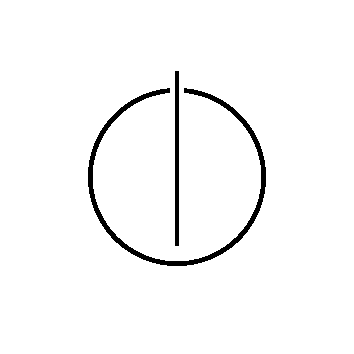
\includegraphics[width=4cm]{styles/informat.png}
  \end{figure}
  
  \end{center}
%	\clearemptydoublepage
%	
%	% The titlepage for the CAMP report document.
% Included by MAIN.TEX


%--------------------------------------------------
% The title page
%--------------------------------------------------

% correct BCOR - undo at the end !!!
\def\bcorcor{0.15cm}
\addtolength{\hoffset}{\bcorcor}

\thispagestyle{empty}

 \vspace{10mm}
\begin{center}
	       \oTUM{4cm}
	   
	   \vspace{5mm}     
	   \huge FAKULT{\"A}T F{\"U}R INFORMATIK\\ 
	   \vspace{0.5cm}
	 \large DER TECHNISCHEN UNIVERSIT{\"A}T M{\"U}NCHEN\\
        
	\end{center}
		

\vspace{10mm}
\begin{center}

   {\Large \doctype}

  \vspace{10mm}
  
  {\LARGE \title}\\
  
  
  \vspace{10mm}
  
  
  {\LARGE  \titleGer}\\
  
  
  \vspace{10mm}

    %\hfill
    \begin{tabular}{ll}
	   \Large Author:     & \Large \author \\[2mm]
	   \Large Supervisor:    & \Large Prof. Michael Beetz\\[2mm]				
	   \Large Advisor:	& \Large M.Sc. Dejan Pangercic\\[2mm]
	   \Large Date:       & \Large July 15, 2011
	 \end{tabular}
	 
	 \vspace{5mm}
	 
	 \begin{figure}[h!]
  \centering
   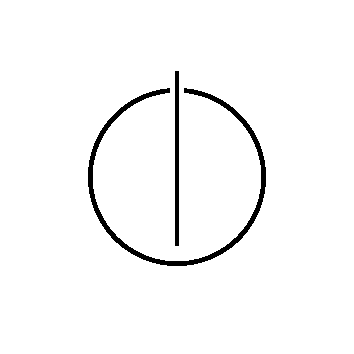
\includegraphics[width=4cm]{styles/informat.png}
  \end{figure}
   

\end{center}

% undo BCOR correction
\addtolength{\hoffset}{\bcorcor}

	
	
%	\input{components/cover_maschmeyer}
	\clearemptydoublepage
	
	% The titlepage for the CAMP report document.
% Included by MAIN.TEX


%--------------------------------------------------
% The title page
%--------------------------------------------------

% correct BCOR - undo at the end !!!
\def\bcorcor{0.15cm}
\addtolength{\hoffset}{\bcorcor}

\thispagestyle{empty}

 \vspace{10mm}
\begin{center}
	       \oTUM{4cm}
	   
	   \vspace{5mm}     
	   \huge FAKULT{\"A}T F{\"U}R INFORMATIK\\ 
	   \vspace{0.5cm}
	 \large DER TECHNISCHEN UNIVERSIT{\"A}T M{\"U}NCHEN\\
        
	\end{center}
		

\vspace{10mm}
\begin{center}

   {\Large \doctype}

  \vspace{10mm}
  
  {\LARGE \title}\\
  
  
  \vspace{10mm}
  
  
  {\LARGE  \titleGer}\\
  
  
  \vspace{10mm}

    %\hfill
    \begin{tabular}{ll}
	   \Large Author:     & \Large \author \\[2mm]
	   \Large Supervisor:    & \Large Prof. Michael Beetz\\[2mm]				
	   \Large Advisor:	& \Large M.Sc. Dejan Pangercic\\[2mm]
	   \Large Date:       & \Large July 15, 2011
	 \end{tabular}
	 
	 \vspace{5mm}
	 
	 \begin{figure}[h!]
  \centering
   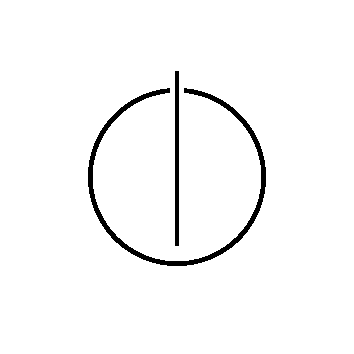
\includegraphics[width=4cm]{styles/informat.png}
  \end{figure}
   

\end{center}

% undo BCOR correction
\addtolength{\hoffset}{\bcorcor}

	
	
	\clearemptydoublepage


\thispagestyle{empty}
\selectlanguage{german}
	\vspace*{0.8\textheight}
	\noindent
	Ich versichere, dass ich diese Bachelorarbeit selbst{\"a}ndig verfasst und nur 
	die angegebenen \\Quellen und Hilfsmittel verwendet habe.
	
	\vspace{15mm}
	\noindent
	M{\"u}nchen, den 15. Juli \hspace{5cm} \author
\selectlanguage{english}
\newpage

	
	\clearemptydoublepage
\phantomsection
\addcontentsline{toc}{chapter}{Acknowledgements}	


%\chapter*{Acknowledgements}

\vspace*{2cm}

\begin{center}
{\Large \bf Acknowledgments}
\end{center}

\vspace{1cm}

\begin{center}
    To my family.
\vspace{1cm}
\end{center}

% M.K.
% L.C.G.
% D.P.
% H.M.A.
% G.A.
% C.S.
% T.R.
% A.S.
% E.R.
% V.R.
% M.C.B.

\vspace{1cm}


My family has patiently supported me during my four-month quest in science and
technology. My appreciation to my equally dear, and loyal friends, who I
certainly have met less often than I would have liked to.  Thanks to Dejan
Pangercic, my advisor, who was the first to introduce me into the challenges to
be found in the world of robotics and computer vision. Lucian Goron was never
short of pragmatic advice. Thumbs up for Manuel Baierl for finding a money- and
time-saving shortcut to the laboratory. The discussions with Martin Kreuzeder
helped to shape my understanding about geometry, proving useful in several
parts of this work.  Many thanks to Hans-Martin Adorf for his generous
comments, and his advice on style.  Thanks to Gabriel Adorf and Christian
Schöne, who both taught me about the importance of graphics, and the basics in
how to create them. Yet, my drawing are no match to theirs. Thanks to Chanrith
Siv for helping me to remove the roughest edges in my English writing. Thanks
to Alexander Shishkov, Ethan Rublee, and Vincent Rabaud for their comments on
software that was not supposed to be used by the public. Notably, the help of
Zoltan-Csaba Marton and Thomas Rühr, who helped me operating the robot at
Technische Universität München. Thank you.


	
	% Abstract for the TUM report document
% Included by MAIN.TEX


\clearemptydoublepage
% Enable when used with hyperref
% \phantomsection
\addcontentsline{toc}{chapter}{Abstract}	

\vspace*{2cm}
\begin{center}
{\Large \bf Abstract}
\end{center}
\vspace{1cm}

Recognition of textured objects is fundamental in many robotic applications in
household environments. This work addresses the perception task of finding a
rigid textured object and its 3D pose in a cluttered scene such that the
cluttered scene can subsequently be resolved by successive removal of objects
by a robot.

A system is presented that learns local 2D features and 3D models from objects.
It is able to detect an object and estimate its pose in a cluttered scene by
matching observed local 2D features against the learned models.  Confidence
values provide a measure of goodness for estimated object poses. For the object
with the highest confidence value, the pose is refined in order to reduce
error, and that estimate provides a basis for the grasping pipeline of a robot.
The system is based on the existing, yet immature and unstable textured object
recognition stack in the Robot Operating System. Recent developments in object
recognition are reviewed in this context, especially the Oriented BRIEF feature
detector and descriptor.

Experiments have shown that in 82\% of cluttered scenes in a validation set, an
object is correctly recognized in the scene within a margin for rotational
error of 20 degrees and for translational error of 3 cm.  A live test on the robot
revealed limitations as well as promising aspects of the approach.

\clearemptydoublepage
% Enable when used with hyperref
% \phantomsection
\addcontentsline{toc}{chapter}{Zusammenfassung}

\vspace*{2cm}
\begin{center}
{\Large \bf Zusammenfassung}
\end{center}
\vspace{1cm}


Die Erkennung von Objekten spielt in vielen Anwendungen der Robotik in
Haushalten eine wichtige Rolle. Diese Arbeit beschreibt die Aufgabe, die Lage
und Orientierung eines starren, texturierten Körpers in einer Szene mit vielen
weiteren Objekten zu bestimmen. Auf diese Art und Weise sollen die Objekte
nacheinander von einem Roboter entfernt werden können.

Ein System wird vorgestellt, welches lokale 2D-Merkmale und 3D-Modelle von
einem Objekt erstellt. Indem das System beobachtete lokale 2D-Merkmale mit den Modellen
assoziiert, kann es ein Objekt erkennen, und dessen Lage und Orientierung im
Raum bestimmen. Konfidenzwerte geben Aufschluss über die Zuverlässigkeit für
die Schätzungen der Lage und der Orientierung der Objekte.  Die erste Schätzung
mit dem höchsten Konfidenzwert wird verfeinert. Die verfeinerte Schätzung
reduziert den Fehler und ermöglicht dem Roboter, das Objekt zu greifen. Das
System beruht auf der bestehenden, noch nicht ausgereiften
Textured-Object-Recognition-Bibliothek aus dem Robot Operating System.  Jüngste
Entwicklungen aus der Objekterkennung werden vorgestellt, insbesondere darunter
der Oriented-BRIEF-Algorithmus zur Bestimmung und Beschreibung von lokalen
2D-Merkmalen.

Experimente zeigen, dass die Lage und die Orientierung eines Objekts in 82\%
der zur Validierung ausgewählten Szenen erfolgreich bestimmt werden, mit einer
Fehlertoleranz von 3 cm Versatz und 20 Grad Winkelunterschied. Ein Testlauf auf
dem Roboter zeigt sowohl Grenzen als auch vielversprechende Aspekte des
Ansatzes auf.



	\tableofcontents
  
  \clearemptydoublepage

\phantomsection
% \addcontentsline{toc}{chapter}{Outline}

\begin{center}
	\huge{Outline}
\end{center}

%--------------------------------------------------------------------
\section*{Part I: Introduction}

\noindent {\scshape Chapter 1: Statement of the Problem}  \vspace{1mm}

The reader learns about the outcome of the work, and about the contribution of
this work to the field. The reader learns about existing other work in this
area.

\noindent {\scshape Chapter 2: Intended Purpose}  \vspace{1mm}

The reader learns why this work has been done and where the system can be used.

\noindent {\scshape Chapter 3: Selected Approach}  \vspace{1mm}

The reader learns about the methods that have been employed.

%--------------------------------------------------------------------
\section*{Part II: Theory}

\noindent {\scshape Chapter 1: Object Recognition}  \vspace{1mm}

The reader learns about the terminology used in object recognition,
especially with regard to this paper. The reader learns about existing work in
object recognition that is important for this work. The reader learns about
different approaches to object recognition.

\noindent {\scshape Chapter 2: Classifier Evaluation}  \vspace{1mm}

The reader learns about the terminology used in classifier evaluation,
especially with regard to this paper. The reader learns about how to view
the object recognition task as a classification problem. 

%--------------------------------------------------------------------
\section*{Part III: Implementation}

\noindent {\scshape Chapter 1: Model Learning}  \vspace{1mm}

The reader learns about how models are generated that lay the foundation for
later classification. The reader learns how certain difficulties have been
resolved. The reader learns about the learning parameters and their effects.

\noindent {\scshape Chapter 2: Object Recognition}  \vspace{1mm}

The reader learns how the classification process works and how the pose of the
object is estimated. The reader learns about the design choices.  The reader
learns about the parameters that can be adjusted to get different classifiers.

\noindent {\scshape Chapter 3: Parameter Selection}  \vspace{1mm}

%--------------------------------------------------------------------
\section*{Part IV: Results}

\noindent {\scshape Chapter 1: Performance in Experiments}  \vspace{1mm}

The reader learns about performance on datasets. The reader learns about how much
influence 3d information in models has on classification. The reader learns about
how long classification takes. 

\noindent {\scshape Chapter 2: Future Work}  \vspace{1mm}

The reader learns which areas have not been sufficiently investigated into,
which issues remain and where to improve.

\noindent {\scshape Chapter 3: Conclusion}  \vspace{1mm}

The reader is reminded what this work was about. The reader learns about what is
different to other works and possible usage scenarios are presented.
% 
% %--------------------------------------------------------------------
% \section*{Part I: Introduction and Theory}
% 
% \noindent {\scshape Chapter 1: Introduction}  \vspace{1mm}
% 
% \noindent  This chapter presents an overview of the thesis and it purpose. Furthermore, it will discuss the sense of life in a very general approach.  \\
% 
% \noindent {\scshape Chapter 2: Theory}  \vspace{1mm}
% 
% \noindent  No thesis without theory.   \\
% 
% %--------------------------------------------------------------------
% \section*{Part II: The Real Work}
% 
% \noindent {\scshape Chapter 3: Overview}  \vspace{1mm}
% 
% \noindent  This chapter presents the requirements for the process.


	\mainmatter
	
	
		% ---------------------------------------------------------------------------
		% \part[Introduction]{Introduction}
		\chapter[Introduction]{Introduction}
		\label{chapter:introduction}
		%\chapter{Introduction}
%\label{chapter:introduction}

\section{Intended Purpose}

Recognition of objects is a fundamental problem in computer vision. We present
a system that detects a textured object and finds its pose in a cluttered
scene. A cluttered scene is formed by multiple textured objects that often
partially occlude each other and are only partially visible to the observer.
The intended purpose of this system is to allow a robot to find the pose of an
object pose such that a robot can then resolve the clutter by scene
manipulation. We assume that objects are removed by the robot from the scene
one-by-one, thus our system focuses on robustly finding the pose of a single
object rather than attempting to recognize all objects in the cluttered scene
at once.

The challenges of solving such a task are plenty. Partial occlusion renders the 
task of detecting objects difficult. The objects in the cluttered scene might
be arbitrarily rotated, and we cannot make any prior assumption about their
principal axes.

A possible application of the system is in household environments, such as a
kitchen.  Let us assume that a robot is given the task to go shopping and that
it will empty the shopping bag onto a kitchen table. Cans, bottles and boxes
and many other items from supermarkets are all textured objects. The next step
for the robot is to move all shopping items to appropriate locations in the
kitchen. The shopping items are assumed to be textured objects and they form a
cluttered scene on the kitchen table. Our system will then provide the robot
with sufficient information to remove one of the items from the cluttered
scene. Multiple iterations will allow the robot to fully resolve the scene.

The actual manipulation of the scene by a robot is not part of this work, but
the application provides the constraints and the assumptions of our system. A
textured object shall be recognized with high and measurable confidence, and
also be correctly located within tolerable error bounds.

\section{Related Work}

... xyz did that ... z means this is difficult ... a chose this .. b did something
similar but based on different assumptions ... 

\section{Selected Approach}

Our approach is based on constructing 3d models and extracting local 2d
features from template objects. Local features have significant advantage over
template matching when objects are partially occluded. % TODO: citation Every
Given a query image, we then match local 2d features to obtain a mapping
between 2d keypoints that belong to the query image and 3d points from the
previously learned template model. We then generate estimates for the object
poses on the query image based on Random Sample Consensus (RANSAC). The pose
that is supported by the highest number of matches is then refined by a second
cascaded classifier that has only been trained on the single object. Each
estimate is assigned a confidence probability that has been learned on ground
truth data. In case the ground truth data is sufficiently similar to the data
encountered in applications, this confidence probability might be used for
selecting a trade-off between true and false positive rates.% TODO: Zitat Fawcett 2006


		
		% ---------------------------------------------------------------------------
		\chapter[Theory]{Theory}
		\label{chapter:theory}
        % \chapter{Theory}
% \label{chapter:theory}

\section{Object Recognition}

% \subsubsection{Applications of Object Recognition}
% Mars mission
% Flood detection
% Earthquake detection
% Industrial quality control

Object recognition is the problem of finding or labeling objects in a query
scene.

\subsection{Local Features}

Object recognition using local features is based on the detection of keypoints
in an image. There is a multitude of different methods available, but they all
aim at choosing keypoints that are repeatable for the same object over
different images. A feature consists of a keypoint and a feature descriptor
captures information about the keypoint and the local image neighborhood.  The
distance between two feature descriptors provides a means of measuring
similarity between two features. 

\subsubsection{Feature Detectors}

A feature detector is an algorithm that designates keypoints on an image.  Some
feature detectors assign orientations to keypoints. Detectors can be roughly
partitioned into three groups. First, there are {\it corner detectors}, such as
Harris and SUSAN, that select points with high curvature. Second, {\it blob
detectors} such as SURF or DoG look for points that are surrounded by all
brighter or darker pixels.  Third, there are {\it region detectors}, such as
MSER, which extract features by finding image regions.

There is generally no such thing as the best feature detector. As often in
engineering, all we can do is making the best choice for the task at hand.  An
ideal feature detector though, should be {\it efficient} and it should find
features that are {\it repeatable}, {\it informative}, {\it local}, and {\it
accurate} \cite{Tuytelaars2007}.

Repeatability describes the chances that the same point on an object shown from
two different viewpoints and viewing conditions is detected on both images.
Thus, repeatability is very important when trying to find correspondences
between two images. A feature detector designates keypoints after examining the
local image neighborhood. These neighborhoods can for example be deformed by
noise, image discretization, a change of viewpoint or a change in lighting
conditions \cite{Tuytelaars2007}. These deformations have to be addressed by a
feature detector to achieve repeatability.

An informative feature belongs to an image neighborhood that shows high
variation in intensity. If not, the features would be difficult to distinguish.
For example, we would not like to have features detected on non-textured
background or areas that carry little information.

A local feature only carries information about a small neighborhood. That
ensures that it is still repeatable despite of occlusion. A small neighborhood
also leads to less informative features, enforcing a trade-off between locality
and informativeness.


\subsubsection{Feature Descriptors}

A feature descriptor generally computes a vector that describes the local
neighborhood of a keypoint. Ideally, two corresponding keypoints should have
very similar descriptor vectors, such that correspondences be found by
nearest neighbor search. A feature descriptor that allows for efficient
matching is BRIEF \cite{Calonder2010}. 

\begin{table}
    \begin{center}
        \begin{tabular}{lcccc}
            Detector & Multi-scale & Oriented Keypoints \\
            \hline
            SIFT & yes & yes \\
            SURF & yes & yes \\
            FAST & no & no \\
            ORB & yes & yes 
        \end{tabular}
    \end{center}
    \caption{Properties of selected feature detectors}
\end{table}

\subsection{Feature Matching}

In multi-view object recognition using local features, correspondences between
known views of the object and the query image can be established by matching
features from the query images to the features from the model. Computation time
depends on the size of the descriptor vector, the nearest neighbor algorithm
and the used distance metric. Great speed-ups can be achieved by weakening the
requirements and allowing for approximate nearest neighbors. Computing the
distance between binary features is faster than with real-valued feature
descriptors.

\subsection{SIFT}

The scale-invariant feature transform became popular in object recognition.  It
is desirable that images of objects at different scales produce more or less
the same features. SIFT achieves this by selecting keypoints from a scale-space
pyramid in order to generate scale-invariant features. SIFT is both a feature
detector and descriptor. Lowe further described a system that lets
correspondences vote in a Hough space, which is dimensioned by location,
orientation and scale \cite{Lowe1999}. When bins contain more than a predefined
number of votes, the object is said to be recognized at this pose.  SIFT was
successfully applied to TODO.

\subsection{Oriented BRIEF}

{\it Oriented BRIEF} or in short {\it ORB} is a combination of the FAST feature
detector and the BRIEF feature descriptor, plus modifications that render the
extracted features orientation-invariant. It was designed to outperform SIFT
and SURF at least in terms of computation time. An implementation is already
available in the development branch (trunk) of OpenCV, a corresponding paper is
expected to be published at ICCV 2011.

FAST is a feature detector based on analyzing Bresenham circles around
candidate keypoints. Generated features are neither orientation nor rotation
invariant.

BRIEF is a binary feature descriptor, which is sensitive to rotation. It
computes a bit string for the image neighborhood of a given keypoint. Each bit
stores the result of the comparison of pixel intensities between two 2-d points
in the neighborhood, which are called {\it test locations}. The test locations
were randomly sampled from a 2-d Gaussian distribution and together form a {\it
test pattern}. Finding nearest neighbors of binary descriptors according to
Hamming distance is faster than for real-valued features using the L2 norm.

% TODO: include image for test locations from orb\_patterns in opencv trunk

ORB computes image moments to define orientation for keypoints detected by
FAST. Image moments of order $(p + q)$ are defined for a 2-d digital image $f$
of dimension $MxN$ as

\begin{equation}
    m_{pq} = \sum_{x=0}^{M-1} \sum_{y=0}^{N-1} x^p y^q f(x, y)
\end{equation}

ORB computes moments $m_{01}$, and $m_{10}$ for neighborhoods $f$ of the
keypoints and designates orientations $\alpha$ as

\begin{equation}
    \alpha = \arctan \frac{m_{01}}{m_{10}}
\end{equation}

Consider the vector $\left( m_{01}, m_{10}\right)^T$. The angle of the vector
becomes the orientation of the keypoint. If $f$ were a probability
distribution, then this vector would contain the means of the marginal
distributions of x and y, respectively.

A problem arises, when rotating the BRIEF test pattern according to the FAST
keypoint orientation. There is correlation between the image moments and the
BRIEF vectors obtained from rotated test patterns. Such correlation reduces
entropy of the BRIEF descriptor. The solution is to compute test patterns that
have only little correlation.

\subsection{Locality Sensitive Hashing}

% TODO: consistent use of uppercase and lowercase in algorithm names

SIFT, ORB and other feature detectors and descriptors are used to describe an
image in terms of local features. Nearest neighbor matching can then find
correspondences between two feature sets. Locality Sensitive Hashing (LSH)
quickly finds nearest neighbors, and trades correctness in favor of a reduction
in computation time. Not always does it return the absolute nearest neighbor.
Locality Sensitive Hashing is a randomized algorithm that performs multiple
scalar projections of a high-dimensional vector and reasons that the scalar
projections are similar for similar input vectors. It can be extended to find
nearest neighbors for binary features. LSH has applications in object
recognition, image retrieval, music rerieval, identification of duplicates
\cite{Slaney2008}.

\section{Pose Estimation}

\subsection{Rigid Transformations}

A {\it rigid transformation} is defined as combination of an orthogonal
transformation and translation in Euclidean space. A {\it proper rigid
transformation} requires the orthogonal transformation to be a rotation. In
three dimensions, a proper rigid transformation can be represented by a
rotation matrix $R \in \mathbb{R}^3$ and a translation vector $t \in
\mathbb{R}^3$.

\begin{equation}
    T: \mathbb{R}^3 \to \mathbb{R}^3, v \mapsto Rv + t
\end{equation}

A proper rigid transformation can be used to describe a rigid motion of an
object. It can also be used to transform the coordinate systems, whilst objects
in the scene remain unchanged with respect to a fixed world frame. The latter
interpretation is prevalent in this work.


\subsection{Hough Transform}

\subsection{RANSAC}

RANSAC stands for {\it RANdom SAmple Consensus} and is a randomized algorithm
that fits a parametrized model to given data. It is robust to outliers, and
therefore a replacement for least-squares fitting in applications that have to
deal with lots of noise. RANSAC randomly chooses the minimal set of data points
that fully determine the model parameters. Then it forms a consensus set out of
all data points that are consistent with the model up to a certain margin of
error. RANSAC constructs a fixed number of such consensus sets and then chooses 
the model with the largest consensus as an estimate.

One application of RANSAC is pose estimation. There are six degrees of freedom
for an object to be located and oriented in space, three for translation and
three for orientation. Three points in a 2-d perspective projection are
necessary and sufficient to determine a pose. If there were no noise in the set
of 2-d correspondences, we would be able to find poses of an object by simply
taking any three correspondences belonging to this object. Unfortunately, image
noise, discretization effects and approximate nearest neighbors asks for a more
sophisticated approach that incorporates strategies to deal with noise and
inconsistency. RANSAC iteratively selects three correspondences to compute pose
estimates. The 3-d model of the template object at the estimated pose is then
back-projected on the query image to compute the projection error and the
consensus set.

\section{Machine Learning}

\subsection{Classification}

\subsection{Estimation}

\subsection{Recognition}

\subsection{Parameter Optimization}



	
		% ---------------------------------------------------------------------------
		\chapter[Implementation]{Implementation}
		\label{chapter:implementation}
        % \chapter{Implementation}
% \label{chapter:implementation}

\section{Model Learning}

\section{Object Recognition}

\section{Parameter Selection}

% see: Alpaydin: Introduction to Machine Learning
As we had the choice between several keypoint detection algorithms, matching
algorithms and each algorithm coming with a set of controllable parameters, we
were facing the difficulty of choosing a configuration that serves our purpose.
The way we look at the problem and the terminology used was heavily influenced
by "Decision and Estimation Theory" (Melsa and Cohn) and by "Introduction to
Machine Learning" (Alpaydin).

In order to do the parameter selection properly, we have to fit our problem
into a mathematical model. This turned out to be more difficult than expected.
Both recognizing an object and correctly locating it within a scene is no
longer a pure classification task. It is not a regression task either. Yet, it
turned out that it is possible to view this problem as an estimation problem,
where we want to estimate the 6 degrees of freedom that uniquely define
location and orientation of an object in space. We follow the model introduced
in Melsa \& Cohn. Let us first consider one object in a scene only (e.g. we
know it's haltbare\_milch). The object and its pose form a {\it message}. There
are infinitely many poses and therefore the {\it message space} is infinite. If
we had access to the full undistorted {\it signal}, there would be absolutely
zero difficulty in estimating the pose.  When we try to find its pose, we have
to derive an estimation based on our {\it observation}. This observation
represents only distorted parts of the signal due to occlusion, perspective,
noise introduced by sensors and unknown variables such as lighting conditions.
\begin{itemize}
\item multiple objects?
\item background?
\item what is the signal exactly?
\item what is the observation exactly?
\end{itemize}
It was therefore natural to define a measure that allowed us to compare
different configurations. This measure is called {\it response}. We defined the
response to depend on the error between estimated pose and ground truth. We
chose to incorporate the notion of approximately correct pose estimates into
the response. That way we avoid having to make a binary choice between correct
and wrong estimate, and leads to more fine-grained responses that retain more
information about test results.

Consider a set of scenes $S$ for which ground truth is available. Given k
parameters $\theta_1, ..., \theta_k$ that represent our choice of algorithms
and the parameters of these algorithms, we define the response for a given set
as a function $r: S \mapsto r (S|\theta)$. In the next step, we can maximize
the response for a given set by altering the parameters $\theta$.



% Note that the problem of detecting an object in the scene by just tagging the
% image is a pure classification task. 




		% ---------------------------------------------------------------------------
		\chapter[Results]{Results}
		\label{chapter:results}
        % \chapter{Results}
% \label{chapter:results}

\section{Performance in Experiments}
\section{Future Work}
\section{Conclusion}


		% ---------------------------------------------------------------------------
		\chapter[Bonanza]{Bonanza}
		\label{chapter:bonanza}
        

How tod\_training works

This is a summary of how tod\_training works, describing input, steps,
algorithms and the output of the training process.

See also http://answers.ros.org/question/289/does-tod\_training-in-object\_recognition-require

See also http://answers.ros.org/question/505/purpose-of-pose-estimations-in-tod\_detecting

See also http://answers.ros.org/question/504/physical-setup-for-collecting-tod\_training-data

% TODO: Learning NOT training

% TODO: replace "training subject" with "template"
% TODO: replace "training" with "learning"
% TODO: find name for "estimated pose" 
% TODO: find name for "guessed pose" 
% TODO: can we say "guess" or better "estimate" or neither?
\begin{description}
    \item[training]the process of creating a training base
    \item[training base] the database that contains the learned classifier for recognition
    \item[training pipeline] the different stages involved in the training process
    \item[training subject] the object to learn to be recognized by the system
    \item[view] shows a training subject in a certain pose
    \item[training image] a per-view 2d image that shows the training subject in a specific pose
    \item[training cloud] a per-view 3d point cloud sampled from the training subject
    \item[estimated pose] an estimate of translation and rotation of the training subject in a view
    \item[masking] extracting the region of interest in the training image
    \item[feature detection] the selection of keypoints in an image
    \item[feature extraction] the generation of feature descriptors for keypoints
    \item[keypoint] a (hopefully) characteristic point in an image
    \item[keypoint descriptor] a vector that describes the characteristics of a keypoint
    \item[training keypoint] a keypoint in a training image
    \item[query image] a test image on which objects shall be detected
    \item[query keypoint] a keypoint in the query image
    \item[recognition] the process of detecting objects in an image
    \item[match] a pair of a query keypoint and a training keypoint with similar descriptors
    \item[guess] an estimate that an object is shown on the query image, including pose
    \item[guessed pose] the fitted pose estimate for an object detected in a query image
    \item[inlier] A matching query keypoint that supports the guessed pose.
\end{description}

\section*{Overview over training pipeline}

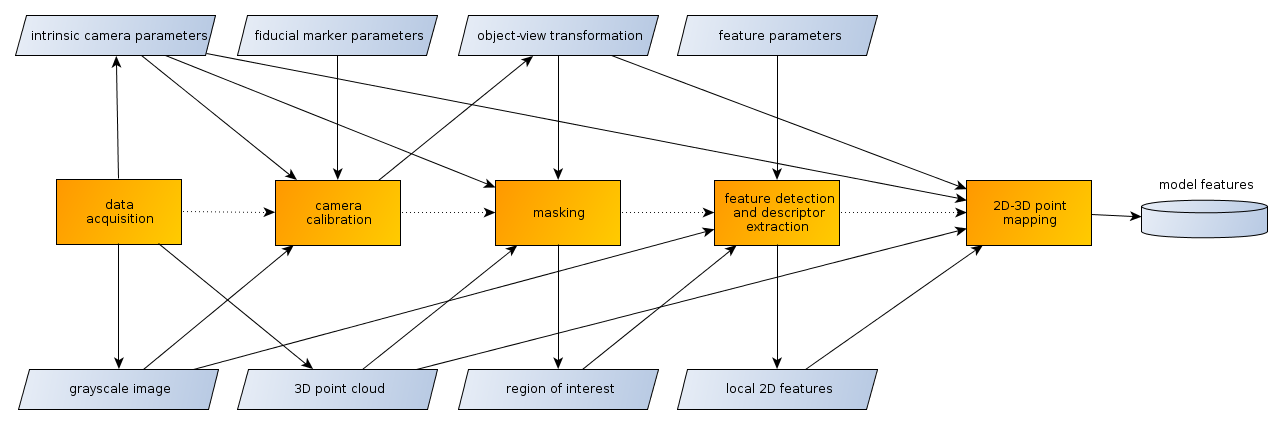
\includegraphics[width=\textwidth]{../doc/tod_training}

Yellow boxes represent processes/steps/actions and grey boxes represent data
artifacts used by or created in the different steps.

\section*{Input data}

The tutorial http://www.ros.org/wiki/tod\_training/Tutorials/BaseCreation
provides links to the training bags found in
http://vault.willowgarage.com/wgdata1/vol1/tod\_kinect\_bags/training/. These
training bags contain the following information

camera\_info     sensor\_msgs/CameraInfo

image               sensor\_msgs/Image

points2         sensor\_msgs/PointCloud2

(image\_mono sensor\_msgs/Image)

(tf                 tf/tfMessage)

According to the tutorial the topics camera\_info, image and points2 are
absolutely necessary and the training subjects or the rotating platform they
are placed upon have fiducial markers rigidly attached to them.

\section*{Training base preparation}

\subsection*{Bag dumping}

Before starting the actual training, it is necessary
to extract information from the compressed bag files and bring this data into a
certain directory layout. The responsible script is dump\_all.py which
delegates the preparation work to bag\_dumper.cpp. It uncompresses the
obligatory point clouds, images and camera information from the recorded bag
files to the directory which is referred to as the training base. The topic
names can be remapped via command-line. Note: at the time of writing, the bag
dumping tool was broken, see 5082 for a workaround.



\subsection*{Training process}

The training process is triggered by train\_all.sh which runs a training
pipeline for each training subject. We can derive the four steps from
train\_object.sh. The different stages in the pipeline pass results as files.
The four steps are:

\begin{enumerate}
    \item Pose estimation (apps/pose\_estimator.cpp)
    \item Masking (apps/masker.cpp)
    \item Feature detection and extraction  (apps/detector.cpp)
    \item 2d-3d point mapping  (apps/f3d\_creator.cpp)
\end{enumerate}

It is crucial to find out what every single of these steps does, which input
they require and what output they produce. As the results are implicitly passed
between the different training stages, this is a little bit more complicated.


\subsubsection*{Pose estimation}

The goal of the pose estimation step is to find the pose (6d) of the training
subject for each training image and save this pose in a yaml file that
corresponds to a training image.

Input
\begin{itemize}
    \item a training image
    \item a description about the fiducial marker
    \item camera information
\end{itemize}

Output
\begin{itemize}
    \item pose estimation for the training image
\end{itemize}

The pose estimation is performed by FiducialPoseEstimator (see pose.h and
pose.cpp) which takes camera information and the training image (which is
converted into a gray-level image) and returns an estimated pose. The list of
images for the training subject is retrieved from a directory listing (see
Opts.cpp), the description of the fiducial marker is read from fiducial.yaml.
The estimated pose is 6-dimensional and consists of a translation and a
rotation vector. You can visualize the estimated pose by enabling the verbosity
option.

If the pose cannot be retrieved from the original image because the corners
of the chessboard could not be detected, there is a fallback to an image that
has been dithered and converted into grayscale using imagemagick's monochrome
operator.

\subsubsection*{Masking}

The masking step extracts the region of interest. The default method used in
tod\_training is based on point cloud segmentation, but makes use of the pose
estimation from the previous step. It reads in the pose information from the
.pose.yaml files generated by apps/pose\_estimator.cpp. Have a look at
apps/masker.cpp.

Input
\begin{itemize}
    \item a point cloud
    \item estimated pose
    \item camera information
\end{itemize}

Output
\begin{itemize}
    \item a black\&white mask
\end{itemize}

The point cloud segmentation (see pointcloud\_segmentation.cpp) works as
follows: The pose estimated from the fiducial markers becomes the center point
of a rectangular box that is used to extract the 3-dimensional region of
interest. The box shape is hard-coded and cannot be altered without changing
the source code. After retrieving all those points in the point cloud that fall
into this box, outliers are removed (via RadiusOutlierRemoval) that have not
enough neighbors within a certain radius. Using OpenCV the segmented cloud in
the 3-dimensional region of interest is projected (Perspective projection) on a
2-dimensional image which then becomes the black\&white mask that masks the
2-dimensional stereo image. This perspective projection actually requires the
camera pose that is retrieved from the very first step in the training
pipeline. Check out masker.cpp which is giving a clue on where the pose
information enters the stage:

       f2d.camera.pose = pose\_est.estimatePose(Mat());

Note that at several places in the pipeline the pose information is retrieved
by calling estimatePose but there is no estimation done. Instead, the pose
information is read from the generated .pose.yaml files and then returned by an
instance of KnownPoseEstimator which is a kind of fake estimator that only
seems to exist for compliance to interfaces.

The produced black\&white mask is saved to a .mask.png file such that it can be
read in the next stage of the training pipeline.


\subsubsection*{Feature detection and extraction}

This step takes the 2-dimensional stereo image, reduces it to the region of
interest and then generates a feature description according to one of a bunch
of available algorithms. Unfortunately, this stage in the pipeline is full of
misnomers or at least misleading terms and therefore difficult to comprehend.
Furthermore, I cannot understand why such a simple design pattern which is
hidden behind the implementation causes such a mess in the implementation
itself. Maybe it's just my ignorance regarding C++ but apart from that there's
no real necessity to make things look more complex than they are.

Input
\begin{itemize}
    \item 2d region of interest as a black\&white mask
    \item 2d gray-scale image
    \item feature extractor configuration
\end{itemize}

Output
\begin{itemize}
    \item a feature description for the 2d gray-scale image
\end{itemize}


Looking into apps/detector.cpp, we can see that it first reads the stereo image
as gray-scale. The color information is not included into the feature
description (which would probably be a bad idea anyway since color information
is very much subject to illumination). Then, a feature detector and a feature
extractor is built according to the parameters specified in
features.config.yaml. This configuration file is compulsory. The feature
extractor populates an instance of Features2d. The feature description will be
stored in a per-view .features.yaml.gz file and the contents are
human-readable. Also, the pose information is read again but it is not really
necessary for the detection process. Instead, the pose information is just
duplicated and stored into an instance of Features2d and finally also ends up
in the .features.yaml.gz file. Evidence for this can be found both in
apps/detector.cpp and in feature\_extraction.cpp where the camera instance of
the Feature2d instance is never used (though the interface would allow to do
so). * Thus, the detector does not use pose information for feature detection
and extraction!

So basically, there are two sub-tasks in this stage. Detection of features and
extraction of features. The detection process finds keypoints in the image and
the extraction process creates a feature description out of these keypoints.

There are several algorithms available, for a up-to-date listing see
feature\_extraction.cpp. At the time of writing, the available detectors
include: FAST, DynamicFAST, SURF, DynamicSURF, STAR, DynamicSTAR, SIFT, MSER
and GFTT. % no longer up-to-date

For feature extraction, tod\_training seems to support: ORB, multi-scale,
sequential, rBRIEF. I cannot say much more at the moment. % no longer up-to-date

\subsubsection*{2d-3d point mapping}

This stage maps the 2d training keypoints to 3d points by projecting the
training cloud onto the 2d image plane and pairing each keypoint with the 3d
point whose projection is closest to that keypoint.

\subsubsection*{Key data structures}

There are several data structures that appear all over the source code in
tod\_training. There are Features2d, Camera, PoseRT.

The Features2d instance has the following members
\begin{itemize}
    \item keypoints
    \item descriptors
    \item image
    \item image\_name
    \item mask\_name
    \item camera (including camera.pose!)
\end{itemize}

Which of those members are currently initialized or not seems to differ
depending on the context where those Feature2d instances are used. Also,
deriving from comments in the source, the developers are not completely sure
about the responsibilities.

The Features2d object has a camera and the camera again stores the pose object,
which is a little bit confusing since intuitively the pose belongs to the
object when seen from the camera coordinate system. Don't get confused. The
camera instance just stores the pose information that is necessary to transform
points between the object coordinate system (draw axes on the objects will
produce this system) and the camera coordinate system (given by the camera
where z denotes what we commonly refer to as depth in space). Have a look at
this picture:

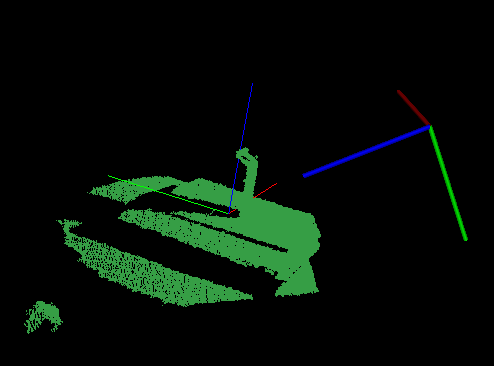
\includegraphics[width=0.7\textwidth]{../doc/pose.png}

\subsubsection*{Output}

The training results are stored in files in a directory which I call the
training base. This training base contains one subdirectory per object.

\begin{verbatim}
config.txt                  List of all objects in the training base.
config.yaml                     Configuration used by tod_detecting
features.config.yaml                Configuration used by tod_training
fiducial.yml                    Description of the fiducial marker.
...
fat_free_milk/                  One folder per object
    camera.yml              Camera information
           ...
           image_00052.png          full color image
image_00052.png.f3d.yaml.gz compressed feature description incl. pose
image_00052.features.yaml.gz    compressed feature description incl. pose
image_00052.png.mask.png               black and white mask   
image_00052.png.pose.yaml              pose information
...
...
\end{verbatim}

\subsection*{How tod\_detecting works}

This is a summary of how tod\_detecting works, which input it requires, which
steps it performs, which algorithms it employs and what the results look like.
The detection of objects in a query image can be roughly separated into four
different subtasks: Reading the training base, extracting features in the query
image, create a matcher.

Some of the files in the training base are no longer of interest, such as the
mask (.mask.png files are not read by tod\_detecting). Also, the png images in
the training base are (as expected) not required by the detection process. All
data the recognizer needs is included in the feature descriptors, the cloud
files and the pose estimations.

See also http://answers.ros.org/question/289/does-tod\_training-in-object\_recognition-require
See also http://answers.ros.org/question/505/purpose-of-pose-estimations-in-tod\_detecting
For collecting training bags, see http://answers.ros.org/question/504/physical-setup-for-collecting-tod\_training-data
and http://answers.ros.org/question/355/recording-a-tod\_training-bag, and http://www.ros.org/wiki/tod\_training/Tutorials/BaseCreation?action=recall\&rev=17.
(this is an old version of the tutorial which includes some information the old
one does not have, Alexander Shikhov pulled this out of the ashes, see for more
information on fiducial markers)

Summary of steps included in recognition process
\begin{enumerate}
    \item Detect and extract features
    \item Matching keypoints
    \item Guessing
\end{enumerate}


This description is about SVN revision 50321. Most of tod\_detecting has changed
since the time of writing, and especially the part about the guessing has been
radically altered.

\subsubsection*{Overview over recognition process}

Yellow boxes represent processes/steps/actions and grey boxes represent data
artifacts used by or created in the different steps.

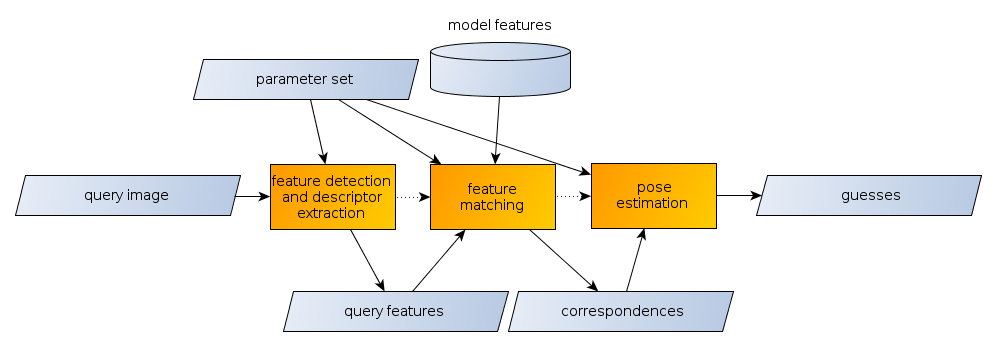
\includegraphics[width=0.8\textwidth]{../doc/tod_detecting_kinect}

\subsubsection*·{Reading training base}

The subjects in the training base MUST be listed in config.txt, subjects not
listed in this file are simply ignored by tod\_detecting. The different training
images for a specific subject are retrieved by looking into sub-folders of the
training base. Such a folder belongs to the training base if it contains a file
called camera.yaml. See recognizer.cpp and Loader.cpp.

For each object, this process consists of
\begin{enumerate}
    \item Loading the pose information for each view
    \item Selecting some of the views based on whether the angles between two successive views exceeds some threshold
    \item For the selected views, load the Feature3d instances from the .f3d.yaml.gz files which also includes the point cloud belonging to this view
\end{enumerate}


\subsubsection*{Detect and extract features}

According to the parameters given in config.yaml, tod\_detecting detects and
extracts features from the query image and stores them in a Features2d
instance. When comparing recognizer.cpp in tod\_detecting and detector.cpp in
tod\_training, we can see that the feature detection and extraction process is
the same, and the code meets expectations that the data prior to matching has
been collected in a similar manner. A working example configuration for feature
detection and extraction is:

detector\_type:   DynamicFAST

descriptor\_type: rBRIEF

extractor\_type:  multi-scale

Using this sample configuration, the classes DynamicAdaptedFeatureDetector,
RBriefFastAdjuster and RBriefDescriptorExtractor, MultiscaleExtractor all come
into play. The feature detection and extraction step does not use pose
information, as both code analysis and GNU debugger show. This is also
symmetrical to what we find in tod\_training.


\subsubsection*{Matching}

Matching is about finding good matches between keypoints in the query and the
training images. The matching is unscrupulously performed between the one query
image and the training images of all training subjects. The result of the
matching is therefore a set of matches between keypoints in the query image and
any training image in the training base.

There are different matching algorithms available, all of them implemented in
OpenCV: FLANN, BF, BF-BINARY,  LSH-BINARY as can be seen in Matcher.cpp. The
parameters can be set in config.yaml and a working example configuration for
the matching process is matcher type:

LSH-BINARY

ratioThreshold: 0.8

knn:  3

doRatioTest: 1

This sample configuration will involve LshMatcher and RatioTestMatcher to
perform the matching.

There are two brute force matchers from OpenCV available that use Manhattan
(BF) or Hamming (BF-BINARY) distance. LSH-BINARY implements  locality sensitive
matching and it is also possible to use a FLANN-based matcher.

The source code is quite chaotic, especially the naming is dubious seen from an
OOP perspective.  One reason is that the tod::Matcher keeps a large parallel
array instead of keeping one list of records. Also, there is a lot of (call it
awesome or obfuscating) book-keeping code involved that deals with different
indices and mapping between those.

The matching process tries to find matches between keypoint descriptors in the
query image and the train images. OpenCV's DescriptorMatcher is used to - find
the k best matches for each keypoint descriptor in the query image and the
keypoint descriptors of the training images. It's performed using some
k-nearest-neighbors algorithm in OpenCV. A cv::DMatch describes such a match
between a query keypoint descriptor and a training keypoint descriptor. The
Matcher is responsible for keeping track of which match belongs to which object
and corresponds to which training image. One query keypoint can find many
matching template keypoints. 


Matcher parameters

See
\begin{description}
    \item[matcher\_type] Specifies which matcher implementation to use. Choose
        between FLANN, BF, BF-BINARY, LSH-BINARY.  See Matcher.cpp
    \item[ratio\_threshold] Used by RatioTestMatcher. See SIFT paper from Lowe 99. See Matcher.cpp
    \item[knn] defines the number of nearest neighbors to find for each query
        keypoint. Equal to parameter k in OpenCV's knnMatch. Must be greater than 1.
        Setting knn = 30 (was 3) produced less positives on ias\_kinect\_test\_all, and
        knn = 100 even less. See Matcher.cpp
    \item[do\_ratio\_test] If true, some pruning and a ratio test is performed.
        See SIFT paper from Lowe 99.  Turning off ratio test lead to far more
        guesses and positives on ias\_kinect\_test\_all.
\end{description}


\subsubsection*{Guessing}

Guessing is the process of actually predicting which training subject can be
found in which pose on the query image. There are two different modes, you can
either use TODRecognizer or KinectRecognizer in Recognizer.cpp and according to
information from Alexander Shikhov, the recognizers differ in performance when
used either with a 5 megapixel Prosilica camera or with a Kinect camera.
Experiments have shown that TODRecognizer and KinectRecognizer perform pretty
much the same in SVN revision 50321, yet KinectRecognizer produces less false
positives on the TOD kinect data set. In SVN revision 50846, KinectRecognizer
has not improved in performance.

\begin{tabular}{ l r c c l }
  Recognizer & SVN revision & Uses Pose & Offers 3d-3d RANSAC & Comments \\
  TODRecognizer & 50321 & No & No & Just uses clustering of keypoints and then RANSAC. \\
  TODRecognizer & 50846 & Yes & Yes & Operates the same way as KinectRecognizer but uses clustering first. See KinectRecognizer::match, TODRecognizer::match and GuessGenerator::calculateGuesses method. \\
  KinectRecognizer & 50321 & Yes & No & Uses 2d-3d model fitting using RANSAC. \\
  KinectRecognizer & 50846 & Yes & Yes & Offers 3d-3d model fitting using RANSAC which is automatically used if a query point cloud is provided, otherwise uses 2d-3d model fitting using RANSAC, just like in older revisions. \\
\end{tabular}


Since TODRecognizer seems to be mostly neglected by the developers of tod\_*,
the following part will only describe KinectRecognizer in 50648.

The Recognizer uses the matcher to find correspondences between keypoint
descriptors in the query image and training images. A tod::Recognizer uses a
tod::Matcher which uses a cv::DescriptorMatcher to first collect a set of
cv::DMatch objects. This set provides the foundation for the whole further
process. A match connects a keypoint in the query image with a matching
keypoint in one of the training images. As such, the matches describe
similarities between the query image and the training images. The following
figure illustrates this relation:

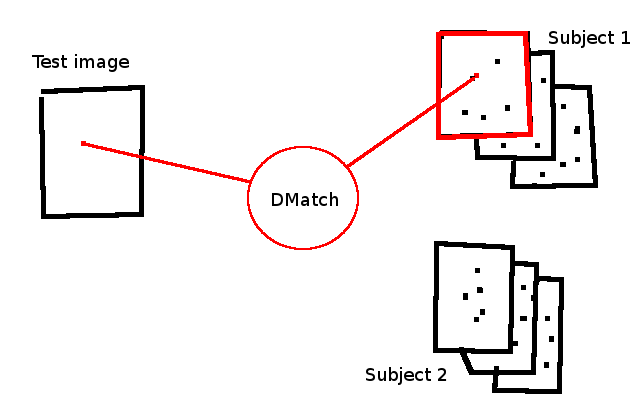
\includegraphics[width=0.8\textwidth]{../doc/dmatch}

The result of the matching is a set of matches. This set contains matches that
link query keypoints with keypoints from different training images. Let this
set of matches be called M.

The idea of the guessing process is now to generate guesses out of these
matches. The simplest solution with questionable performance would probably
consist of simple voting. tod\_detecting takes another approach.

KinectRecognizer iterates over each training subject and looks for possible
occurrences on the query image. Let MS  be the set of all matches on training
images of subject S. KinectRecognizer uses RANSAC to find a pose that minimizes
error between the reprojection of matching 3d points in the training views of S
and the query keypoints. If RANSAC produces enough inliers (i.e. above a
certain threshold referred to as min\_inliers\_count or minInliersCount in the
sources), the algorithm concludes that an instance of training subject S has
been found in the scene. In each training view, there is a one-to-one mapping
between the training keypoints and corresponding 3d points (f3d\_creator). As
such, a match does not only create a correspondence between a query keypoint
and a keypoint in the training image but also links a query keypoint with a 3d
point from the training view. All matches from MS are considered at once when
producing a new guess candidate. The corresponding 3d points are merged into a
common coordinate system according to the pose information gathered in the
training process (pose\_estimator.cpp). We can think of those 3d points forming
a partial 3d model of the training subject that is then being fit to the 2d
projection of the subject in the training image by RANSAC.

Unfortunately, both KinectRecognizer and TODRecognizer use the camera matrix
and the camera distortion matrix used for guessing the pose are taken from the
training images instead of the query image. This is a conceptual mistake that
has to be addressed by filling in the information of the camera used in
testing.


{\definecolor{gray}{rgb}{0.6,0.6,0.6} \color{gray}

TODRecognizer   obsolete

On a per-subject basis, TODRecognizer performs agglomerative hierarchical
clustering of test image keypoints that have been matched with the specific
training subject. At the beginning of the clustering a cluster is created
(remember every keypoint has a keypoint descriptor) for every keypoint in the
test image that found a match in one of the training images. A Cluster consists
of a set of keypoints. The result of the clustering process is a 2-dimensional
Iliffe vector that shows the association between clusters (first index) and the
keypoints (as a list of indices). In order to visualize these clusters, call

drawClusters(test.image.clone(), points, clusterIndices);

where points refers to the test image keypoints mentioned above and
clusterIndices to the Iliffe vector mentioned above.

Then, also on a per-subject basis, a GuessGenerator makes guesses based on the
obtained clusters, the test image and its keypoints and the matches between
keypoints of the test image and the specific subject's training images (often
referred to as objectMatches in the source code). The guesses are
post-processed and filtered according to a criterion based on the standard
deviation of point clouds and some OverlappingFilter I haven't looked into yet.

The GuessGenerator constructs a Features2d and a Features3d instance using the
supplied test image and its keypoints. It remains a puzzle why these Features2d
instances are always constructed on-the-fly and then split into their members
in a manner that appears quite random to me. The number of parameters for each
method is too large. 

--- This part only applies to TODRecognizer in some SVN revision different from
50321. Guesses are calculated separately for each cluster. Multiple guesses can
be generated from one cluster.

For each cluster, every test image keypoint belonging to this cluster is
examined. 2d-to-3d-mode is enabled (I don't know what this is at the time of
writing). At this time, the per-subject-view Features3d instance becomes
important. Citing the documentation of Features3d:

'Encapsulates the relationship between a cloud and a 2d keypoints'                      

'The cloud should have a one to one correspondence with the features.'

For each of the test image keypoints in the cluster, the 3d point from the
training subject's view that corresponds to this keypoint is selected and
transformed using the view-specific inverted (see Tools) pose estimation. So, a
list of 2d keypoints and corresponding 3d keypoints is obtained. Now, RANSAC
(using vslam's solvePnPRansac, which again uses OpenCV's solvePnP, parallelized
with Intel Threading Building Blocks). The documentation of solvePnP says
'Finds the object pose from the 3D-2D point correspondences' and that's what
happening in tod\_detecting.

Note: it seems that recent revisions (e.g. 50470) (also) implement 3d to 3d
matching via RANSAC

The GuessGenerator makes use of the pose estimation obtained in the training
pipeline!

A guess is made if the number of inliers produced by solvePnP exceeds a
threshold and when solvePnP produced a valid pose estimation. If solvePnP fails
to produce a good-quality matching where quality is measured in terms of the
number of inliers, then there will no more guesses be generated for this
cluster. If a guess is made, the remaining keypoints that correspond to
outliers are considered for the next guess.  ---

tod\_detecting uses four methods to distinguish between good and bad guesses?
clusters with not enough keypoints are discarded right away
(min\_cluster\_size, TODRecognizer only) measuring number of inliers produced
by solvePnP (min\_inliers\_count)

filter based on overlapping (TODRecognizer only)

filter based on standard deviation (TODRecognizer only)

The guesses are post-processed and solvePnPRansac is again used to estimate
pose of the object in the test image, but this time only inliers from the
previous solvePnP run are taken into account. The GuessClarifier does not
filter guesses. This seems to be just some optimization.

In SVN revision 50321 we have another version of TODRecognizer. It does not
care about the pose estimations at all.
}

Guess parameters

\begin{description}
    \item[minInliersCount] If number of inliers produced by RANSAC when trying
    to fit a pose is less than minInliersCount, then no guess will be made
    (reject). I expect that increasing minInliersCount will push the classifier to
    the lower left in ROC space and will make false positives less likely.  Must be
    greater than zero. Having set minInliersCount = 1 (was 5) produces hundreds of
    guesses for ias\_kinect\_test\_all. Having set minInliersCount = 10 will
    produce only a few positives (on ias\_kinect\_test\_all). See GuessGenerator.cpp
    \item[ransacIterationsCount] Maximum number of iterations that RANSAC is
    allowed to perform when finding a pose that fits to the keypoints.  Setting
    ransacIterationsCount = 200 (was 100) leads to more positives. Setting
    ransacIterationsCount = 1000 leads to even more positives (50\% true positives
    instead of 20\%, can say nothing about false positives) and more guesses per
    subject, but also starts to slow down recognition (on ias\_kinect\_test\_all).
    See GuessGenerator.cpp pnp\_ransac.cpp
    \item[maxProjectionError] Defines a radius such that RANSAC can distinguish
    between inliers and outliers. When RANSAC finds a hypothetical pose, it uses
    this pose to project 3d points. If the distance between a projected point and
    its corresponding test keypoint is smaller than maxProjectionError.
    Setting maxProjectionError = 20 (was 6) leads to way more guesses and
    positives. Setting maxProjectionError = 1 (on ias\_kinect\_test\_all) results in
    almost zero positives.  See GuessGenerator.cpp pnp\_ransac.cpp
    \item[descriptorDistanceThreshold] Not used at all in whole stack
    object\_recognition, seems to be obsolete, see ticket 5096. See GuessGenerator.cpp
    \item[minStddevFactor] Only used by TODRecognizer, see GuessGenerator.cpp
    Recognizer.cpp.
    \item[minClusterSize] Only used by TODRecognizer. See GuessGenerator.cpp.
\end{description}

When using KinectRecognizer we have the following influential degrees of
freedom for the guessing process: minInliersCount, ransacIterationsCount,
maxProjectionError. The parameter configuration that has been used to create
the training base and detect keypoints and descriptors also influences
performance.



\subsubsection*{Key data structures}
Guess
A guess consists of
\begin{itemize}
    \item the aligned pose of the object in the query image
    \item a standard deviation value
    \item the query image
    \item the recognized textured object
    \item camera calibration and distortion matrix
    \item 2d keypoints on the query image that found a match in a training image
    \item 3d keypoints corresponding to the 2d keypoints in training images that were matched with the query image
    \item inlier points from RANSAC
\end{itemize}

Features2d, Features3d



		
		% ---------------------------------------------------------------------------
		%
		% Appendix
		%
		% ---------------------------------------------------------------------------
		
		\part*{Appendix}
		\addcontentsline{toc}{part}{Appendix}
		
		\appendix %---------------------------------------
		
		% \chapter{Terms}
% \label{chapter:terms}
% 
% \begin{description}
%    \item[template object] a real-world object we want to be able to recognize
%    \item[model] a set of features that describes a template object
%    \item[model view] a 2d image and a point cloud that show a template object from a certain camera viewpoint
%    \item[model image] the 2d image belonging to a model view
%    \item[model cloud] a point cloud belonging to a model view 
%    \item[model keypoint] a 2d keypoint belonging to a model image 
%    \item[model feature] a 2d keypoint, a corresponding 3d point in model frame, and a descriptor vector
%    \item[model frame] a coordinate system attached to the template object 
%    \item[model coordinates] coordinates relative to the model frame 
%    \item[camera frame] a coordinate system attached to the camera 
%    \item[camera coordinates] coordinates relative to the camera frame 
%    \item[camera origin] origin of camera frame 
%    \item[template pose] Defines the transformation of model coordinates into
%        camera coordinates in a given model view. 
%    \item[estimated pose] Estimate for an object's pose in the query image. The
%        translation vector of the estimated pose is equal to the template origin
%        relative to the camera frame.
%    \item[query image] a test image on which objects are to be recognized 
%    \item[query cloud] a test image on which objects are to be recognized 
%    \item[query keypoint] a 2d keypoint in the query image
%    \item[query feature] a 2d keypoint, a corresponding 3d point in camera frame and a descriptor vector 
%\end{description}

\newglossaryentry{template object}{
    name={template object},
    description={used for learning a model, as opposed to the instances in a query scene}
}

\newglossaryentry{object-view transformation}{
    name={object-view transformation},
    description={transforms coordinates from the object coordinate system into the view coordinate system}
}

\newglossaryentry{view-object transformation}{
    name={view-object transformation},
    description={transforms coordinates from the view coordinate system into the object coordinate system}
}

\newglossaryentry{object coordinate system}{
    name={object coordinate system},
    description={describes the 3D points of an object or a model}
}

\newglossaryentry{view coordinate system}{
    name={view coordinate system},
    description={describes 3D points relative to the camera}
}

\newglossaryentry{fiducial coordinate system}{
    name={fiducial coordinate system},
    description={describes 3D points relative to the fiducial markers}
}

\newglossaryentry{query scene}{
    name={query scene},
    description={a scene under investigation where objects are to be recognized}
}

\newglossaryentry{query image}{
    name={query image},
    description={the image of a query scene taken by the camera}
}

\newglossaryentry{point cloud}{}
\newglossaryentry{pose}{}

\newglossaryentry{guess}{
    name={guess},
    plural={guesses},
    description={a pose estimate for a specific object; has a confidence value}
}

\newglossaryentry{guess ranking}{
    name={guess ranking},
    description={orders guesses by a measure of ``goodness'', for example by confidence value}
}

\newglossaryentry{guess rejection}{
    name={guess rejection},
    description={rejects a guess if it is not ``good'' enough, for example if it has a too low confidence value}
}

\newglossaryentry{guess refinement}{
    name={guess refinement},
    description={tries to estimate the pose of a specific object in the scene as accurate as possible}
}

\newglossaryentry{confidence value}{
    name={confidence value},
    description={size of the consensus set found by RANSAC}
}

\newglossaryentry{query feature}{
    name={query feature},
    description={a local 2D feature extracted from a query image}
}

\newglossaryentry{guess score}{
    name={guess score},
    description={assigns a score that describes the distance of a guess to the ground truth in a scene}
}

\newglossaryentry{model feature}{
    name={model feature},
    description={a local feature; the basic building block for a model of a template object}
}

\newglossaryentry{aligned model}{
    name={aligned model},
    description={a model inserted into the scene with a certain pose}
}

\newglossaryentry{inlier}{
    name={inlier},
    description={a correspondence that is consistent with a pose estimate up to
    a certain margin of error; member of the consensus set returned by RANSAC}
}

\newglossaryentry{feature extraction}{
    name={feature extraction},
    description={detection of a keypoint and
        computation of a descriptor vector from its image neighbourhood}
}
\newglossaryentry{validation set}{}
\newglossaryentry{test set}{}
\newglossaryentry{consensus set}{}
\newglossaryentry{outlier}{}
\newglossaryentry{extrinsic parameters}{}
\newglossaryentry{intrinsic parameters}{}
\newglossaryentry{rigid transformation}{}
\newglossaryentry{proper rigid transformation}{}
\newglossaryentry{correspondence}{
    name=correspondence,
    description={a supposed match between a query feature and a model feature; found by nearest-neighbour search}
}
\newglossaryentry{scene}{}
\newglossaryentry{view}{}



        \printglossary 


  \clearemptydoublepage
  
	\bibliography{bibliography/literature}
	
 
\end{document}

